% Chapter Template
\chapter{Methodology} % Main chapter title

\label{Chapter4} % Change X to a consecutive number; for referencing this chapter elsewhere, use \ref{ChapterX}

This chapter covers the hardware and software setup used for performing the GPS spoofing experiments. Rationalising the choices made and discussing the benefits and
limitations of these selections.

%----------------------------------------------------------------------------------------
%	SECTION 1
%----------------------------------------------------------------------------------------

\section{Testing Methodology}

In this section the method of creating a GPS signal spoofing device is detailed. The main part of this device is the upgradeability of the SDR platform
and in particular the USRP N210 SDR. As previously mentioned the benefit of using an SDR over using an ASIC is that with a new version of software 
new capabilities are available to the device. This could be beneficial to either the spoofer or spoof defense. 

The success of the spoofing was dictated by whether the receiver was able to lock onto the signal and calculate the same location as expected or travel the same path
depending on whether the test is a static or dynamic spoofing test. 

Testing was also performed on the reception of GPS signals. Such that they could be used in Meaconing attacks. Initially there was an attempt to receive a GPS signal using
the GPS-SDR software as proof that the antennae were operational. This was then changed such that the reception was handled directly through GNURadio and the raw
digitised version of the signal was saved to a file such that it could be replayed elsewhere.

%----------------------------------------------------------------------------------------
%	SECTION 2
%----------------------------------------------------------------------------------------

\section{Data Collection}

To see the effectiveness of the GPS spoofing methods experiments were carried out and results were recorded. The success of the experiments were dictated by whether or
not the receiver was reporting false location or timing information. Using an Android phone there is access to the raw GPS information which can be used to determine if
the spoofing signal is being accepted. However, the use of a "maps" program was also used as a way to determine if there was any form of software/hardware anti-spoofing
technique being used post GPS receiver. A simple COTS was also used to log the NMEA sentences from its serial interface. A custom program was generated in order to graph
various outputs from these sentences.

For the purpose of this project just three sentences were used when parsing the log files, "GPGGA", "GPGSV" and "GPRMC". The GP mnemonic is a designation that the
received signal was from GPS. The other constellations have their own designations when using NMEA sentences as dictated by Table \ref{tab:NMEA Mnemonics}. 
GGA (Global Positioning System Fix Data) \footnote{https://www.nmea.org/Assets/20130801 0183 identifier list.pdf} sentences contain information related to the fix of the
GPS signal. The calculated latitude and longitude as well as whether DGPS is being used in the fix, as well as others, as shown in Table \ref{tab:NMEA GGA Struct}.
However, only the latitude and longitude information was used, see Listing \ref{list:GGAParse}.

An example of a GGA sentence is:
\begin{verbatim}
$GPGGA,000056.000,3500.5533,S,13834.1337,E,1,10,0.87,-14.7,M,-0.7,M,,*74
\end{verbatim}

\begin{lstlisting}[language=Python, label=list:GGAParse, caption=Parsing GGA sentences for lattitue and longitude information]
try:
    with open(infile, "r") as nmeaFile:
        for count, line in enumerate(nmeaFile):
            tmp = line.split('*')
            string = tmp[0].split(',')
            msgType = string[0][3:]
            currentTime = datetime.now()
            timestamp2 = (currentTime - startTime).microseconds/1000000

            #
            # Parsing GGA sentences
            #
            elif msgType == "GGA":
                if dataValid:
                    try:
                        latitude = degMin2deg(string[2])
                        longitude = degMin2deg(string[4])
                        if string[3] == 'S':
                            latitude = latitude * -1
                        if string[5] == 'W':
                            longitude = longitude * -1
                        coordinates.append([timestamp2, latitude, longitude])
                    except ValueError:
                        print("No valid coordinates")
                        continue
\end{lstlisting}

\renewcommand{\arraystretch}{1.5}
\begin{table}[!h]
    \begin{center}
        \caption{NMEA GGA Sentence structure}
        \label{tab:NMEA GGA Struct}
        \begin{tabular}{ |m{4cm}|c|p{6cm}| }
            \hline
            \textbf{Field} & \textbf{Example} & \textbf{Description} \\
            \hline
            Message ID & \$GPGGA & GGA Protocol header \\
            \hline
            UTC time & 000056.000 & hhmmss.sss \\
            \hline
            Latitude & 3500.5533 & ddmm.mmmm \\
            \hline
            N/S Indicator & S & N = North, S = South\\
            \hline
            Longitude & 13834.1337 & dddmm.mmmm \\
            \hline
            E/W Indicator & E & E = East, W = West\\
            \hline
            Position Fix Indicator & 1 & 0: Fix not available \newline 1: GPS SPS mode, fix valid \newline 2: DGPS SPS mode, fix valid\\
            \hline
            Satellites used & 10 & \\
            \hline
            HDOP & 0.87 & Horizontal dilution of precision\\
            \hline
            MLS Altitude & -14.7 & Meters \\
            \hline
            Units & M & Meters \\
            \hline
            Geoid separation & -0.7 & Meters \\
            \hline
            Units & M & Meters\\
            \hline
            Age of differential correlation & & Seconds\\
            \hline
            Differential reference station ID & &  \\
            \hline
            Checksum & *74 &  \\
            \hline
            <CR><LF> & & End of message termination \\
            \hline
        \end{tabular}
    \end{center}
\end{table}
\renewcommand{\arraystretch}{1}

The use of GSV (GNSS Satellites in View) sentences allowed for tracking how many and which satellites were in view (SVID) and what the carrier to noise ratio ($\frac{C}{N_0}$) was. This was used to generate the carrier to
noise graphs and were stored in key:value dictionaries, see Listing \ref{list:GSVParse}. Since the sentences can only be a set length as per the standard, multiple successive GSV sentences may need to be sent.

An example of a GSV sentence that is part of a group of 4 is:
\begin{verbatim}
$GPGSV,4,1,13,23,70,156,52,10,69,284,52,20,50,138,,18,49,117,52*73
$GPGSV,4,2,13,27,37,224,52,16,32,276,52,15,26,127,51,26,23,308,51*77
$GPGSV,4,3,13,29,19,038,17,32,18,001,18,44,05,279,,13,02,148,47*75
$GPGSV,4,4,13,193,,,*40
\end{verbatim}

\begin{lstlisting}[language=Python, label=list:GSVParse, caption=Parsing GSV sentences for SVID carrier to noise ratio informaiton]
    try:
        with open(infile, "r") as nmeaFile:
            for count, line in enumerate(nmeaFile):
                tmp = line.split('*')
                string = tmp[0].split(',')
                msgType = string[0][3:]
                currentTime = datetime.now()
                timestamp2 = (currentTime - startTime).microseconds/1000000
    
                #
                # Parsing GSV sentences
                #
                elif msgType == "GSV":
                    NumofMessages = int(string[1])
                    sequenceNumber = int(string[2])
                    satellitesView = int(string[3])
                    satellitesToCalc = satellitesView-(NumofMessages-1)*4 # this will dictate the number the index numbers of final sentence of group
                    if sequenceNumber == 1:
                        timestamp = (currentTime - startTime).microseconds/1000000
                    try:
                        if sequenceNumber < NumofMessages:                        
                            if string[4] not in svSNR:
                                svSNR[string[4]] = [string[7]]
                            else:
                                svSNR[string[4]].append(string[7])
    
                            if string[8] not in svSNR:
                                svSNR[string[8]] = [string[11]]
                            else:
                                svSNR[string[8]].append(string[11])
                        
                            if string[12] not in svSNR:
                                svSNR[string[12]] = [string[15]]
                            else:
                                svSNR[string[12]].append(string[15])
                        
                            if string[16] not in svSNR:
                                svSNR[string[16]] = [string[19]]
                            else:
                                svSNR[string[16]].append(string[19])
                        else:
                            if satellitesToCalc >= 1:
                                if string[4] not in svSNR:
                                    svSNR[string[4]] = [string[7]]
                                else:
                                    svSNR[string[4]].append(string[7])
                            if satellitesToCalc >= 2:
                                if string[8] not in svSNR:
                                    svSNR[string[8]] = [string[11]]
                                else:
                                    svSNR[string[8]].append(string[11])
                            if satellitesToCalc >=3:
                                if string[12] not in svSNR:
                                    svSNR[string[12]] = [string[15]]
                                else:
                                    svSNR[string[12]].append(string[15])
                            if satellitesToCalc == 4:
                                if string[16] not in svSNR:
                                    svSNR[string[16]] = [string[19]]
                                else:
                                    svSNR[string[16]].append(string[19])
                            if satellitesToCalc > 4:
                                raise OverflowError
    
                    except IndexError:
                        pass
                    except OverflowError:
                        print("Computational error occured. Access to a value higher than available attempted")
                    if sequenceNumber == NumofMessages:
                        if svSNR:
                            satellites[timestamp] = svSNR
                        svSNR = {}
    \end{lstlisting}

\renewcommand{\arraystretch}{1.5}
\begin{table}[!h]
    \begin{center}
        \caption{NMEA GSV Sentence structure}
        \label{tab:NMEA GSV Struct}
        \begin{tabular}{ |m{4cm}|c|p{6cm}| }
            \hline
            \textbf{Field} & \textbf{Example} & \textbf{Description} \\
            \hline
            Message ID & \$GPGSV & GSV Protocol header \\
            \hline
            Number of messages & 4 & Number of messages in group \\
            \hline
            Sequence Number & 1 & Message number \\
            \hline
            Satellites in view & 13 & Total number of satellites in view\\
            \hline
            Satellite ID 1 & 23 & PRN number of satellite \\
            \hline
            Elevation 1 & 70 & Elevation in degrees (0-90)\\
            \hline
            Azimuth 1 & 156 & Azimuth in degrees (0-359)\\
            \hline
            SNR 1 & 52 & SNR in dBHz (0-99)\\
            \hline
            Satellite ID 2 & 10 & PRN number of satellite \\
            \hline
            Elevation 2 & 69 & Elevation in degrees (0-90)\\
            \hline
            Azimuth 2 & 284 & Azimuth in degrees (0-359)\\
            \hline
            SNR 2 & 52 & SNR in dBHz (0-99)\\
            \hline
            Satellite ID 3 & 20 & PRN number of satellite \\
            \hline
            Elevation 3 & 50 & Elevation in degrees (0-90)\\
            \hline
            Azimuth 3 & 138 & Azimuth in degrees (0-359)\\
            \hline
            SNR 3 &  & SNR in dBHz (0-99)\\
            \hline
            Satellite ID 4 & 18 & PRN number of satellite \\
            \hline
            Elevation 4 & 49 & Elevation in degrees (0-90)\\
            \hline
            Azimuth 4 & 117 & Azimuth in degrees (0-359)\\
            \hline
            SNR 4 & 52 & SNR in dBHz (0-99)\\
            \hline
            Checksum & *73 &  \\
            \hline
            <CR><LF> & & End of message termination \\
            \hline
        \end{tabular}
    \end{center}
\end{table}
\renewcommand{\arraystretch}{1}

As shown in Table \ref{tab:NMEA RMC Struct} RMC (Recommended Minimum Specific GNSS Data) sentences contain a lot of useful information. However, for the purposes of this
project it was only used in order to check when there is valid positional information, Listing \ref{list:RMCParse}.

\begin{verbatim}
$GPRMC,000118.000,A,3500.4918,S,13834.1369,E,53.66,12.07,300321,,,A*78
\end{verbatim}

\begin{lstlisting}[language=Python, label=list:RMCParse, caption=Parsing RMC sentences for data and fix validity checks]
    try:
        with open(infile, "r") as nmeaFile:
            for count, line in enumerate(nmeaFile):
                tmp = line.split('*')
                string = tmp[0].split(',')
                msgType = string[0][3:]
                currentTime = datetime.now()
                timestamp2 = (currentTime - startTime).microseconds/1000000
    
                #
                # Parsing RMC sentences
                #
                if msgType == "RMC":
                    if not dataValid:
                        if not firstFix:
                            timetofix += 1
                    if string[2] == 'A':
                        dataValid = True
                        if not firstFix:
                            firstFix = True
                    else:
                        dataValid = False
    \end{lstlisting}


\renewcommand{\arraystretch}{1.5}
\begin{table}[!h]
    \begin{center}
        \caption{NMEA RMC Sentence structure}
        \label{tab:NMEA RMC Struct}
        \begin{tabular}{ |m{4cm}|c|p{6cm}| }
            \hline
            \textbf{Field} & \textbf{Example} & \textbf{Description} \\
            \hline
            Message ID & \$GPRMC & RMC Protocol header \\
            \hline
            UTC time & 000118.000 & hhmmss.sss \\
            \hline
            Status & A & A = Valid, V = Not Valid \\
            \hline
            Latitude & 3500.4918 & ddmm.mmmm\\
            \hline
            N/S Indicator & S & N = North, S = South\\
            \hline
            Longitude & 13834.1369 & dddmm.mmmm \\
            \hline
            E/W Indicator & E & E = East, W = West\\
            \hline
            Speed over ground & 53.66 & knots \\
            \hline
            Course over ground & 12.07 & degrees \\
            \hline
            HDOP & 0.87 & Horizontal dilution of precision\\
            \hline
            Date & 300321 & ddmmyy \\
            \hline
            Magnetic Variation &  & Meters \\
            \hline
            Mode & A & A = Autonomous, D = DGPS, E = DR \\
            \hline
            Checksum & *78 &  \\
            \hline
            <CR><LF> & & End of message termination \\
            \hline
        \end{tabular}
    \end{center}
\end{table}
\renewcommand{\arraystretch}{1}

\section{Hardware Setup}
For all experiments the same hardware was used. This included the USRP SDR, laptop and GPS receiver. The laptop was an important piece of equipment since it needed to be
powerful enough to be able to feed the data to the SDR quick enough to avoid the aforementioned under run issues. Towards the end of the project there was a hardware fault
with the Pixel XL phone receiver. This was replaced by the Pixel 4a 5G.

There was no formal decision process for choosing the hardware components since they were all parts that had already been purchased and were in possession of the
supervisor. Having said that some research went into the suitability of the equipment, mainly the SDR. It was found that this was one of the most powerful and most
importantly had one of the most stable clock oscillators available in software defined radios. This made is well suited to GNSS based tasks. Alternatives, like the
RTL-SDR are capable devices for the cost, but only offer reception. Duplex options like the HackRF are also suitable for transmitting high bandwidth signals, however the
on board clock is not stable enough for highly accurate signals like that of GNSS. There was a workaround for this, which included de-soldering the included oscillator and
soldering a more stable part. In future, if access to USRP based SDRs is not available then this would be a very good second option. However, there was access to a better
tool, being the N210, therefore it was chosen. From Ettus, there were two daughtercards that allow access to the desired 1575.42MHz band of the L1 GPS signal, the SBX and
WBX. The SBX was chosen because it was already available. It should be noted that there would be no theoretical difference between either daughtercard since the desired
frequency was not at the extreme of either cards bands. Either card would also be capable of transmitting or receiving on the other bands of GNSS constellations.

To ensure the SDR and PC were able to communicate, an ethernet cable was connected between each device and the IP address of the PC was set to 192.168.10.2/24 as per the
default configuration from the setup documentation. To check if the IP address was correctly set, a command line program was run that would poll the appropriate
interfaces of the PC and check for USRP devices attached, see Figure \ref{fig:UHDFind}. There was also a command line program that allowed for the probing of a
radio to gather information on what daughtercard was installed and other properties, see Figures \ref{fig:UHDProbe1}, \ref{fig:UHDProbe2} and \ref{fig:UHDProbe3}.

\begin{figure}[!h]
    \begin{centering}
        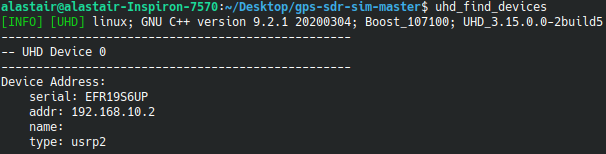
\includegraphics[width=14cm,keepaspectratio]{Figures/uhd-find-devices.png}
        \caption{Using the UHD daemon to find connected USRP SDR devices}
    \label{fig:UHDFind}
    \end{centering}
\end{figure}

\begin{figure}[h]
    \begin{centering}
        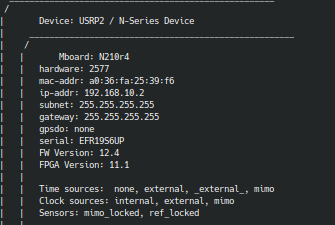
\includegraphics[width=10cm,keepaspectratio]{Figures/usrp-probe-output_1.png}
        \caption{Using the UHD program to probe the hardware details of any connected USRP device. This part of the output shows the main board details}
    \label{fig:UHDProbe1}
    \end{centering}
\end{figure}

\begin{figure}[h]
    \begin{centering}
        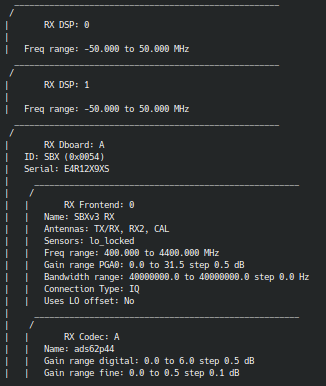
\includegraphics[width=10cm,keepaspectratio]{Figures/usrp-probe-output_2.png}
        \caption{Using the UHD program to probe the hardware details of any connected USRP device. This part of the output shows the reception details}
    \label{fig:UHDProbe2}
    \end{centering}
\end{figure}

\begin{figure}[h]
    \begin{centering}
        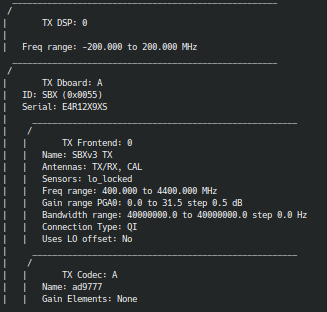
\includegraphics[width=10cm,keepaspectratio]{Figures/usrp-probe-output_3.png}
        \caption{Using the UHD program to probe the hardware details of any connected USRP device. This part of the output shows the transmission details}
    \label{fig:UHDProbe3}
    \end{centering}
\end{figure}

\begin{itemize}
    \item Laptop
    \begin{itemize}
        \item Dell Inspiron 15
        \item CPU: Core i7 Quad Core/ 8 thread
        \item RAM: 32GB
        \item Ethernet Connection: gigabit
    \end{itemize}
    \item Software defined radio
    \begin{itemize}
        \item USRP N210
        \item SBX-40 daughtercard
        \item 30dB attenuator
        \item Full duplex
        \item Gigabit Ethernet connection
        \item high performance FPGA
        \item omnidirectional antenna
    \end{itemize}
    \item GPS Receiver (Phone 1)
    \begin{itemize}
        \item Google Pixel XL
        \item Android 10
        \item Multi constellation GNSS support (GPS+QZSS, GLONASS, BeiDou)
    \end{itemize}
    \item GPS Receiver (Phone 2)
    \begin{itemize}
        \item Google Pixel 4a 5G
        \item Android 11
        \item Multi constellation GNSS support (GPS+QZSS, GLONASS, BeiDou)
    \end{itemize}
    \item GPS Receiver (COTS)
    \begin{itemize}
        \item GPS L1 support only
        \item NMEA output
    \end{itemize}
\end{itemize}

\begin{figure}[!h]
    \begin{centering}
        \includegraphics[width=13cm,keepaspectratio]{Figures/Setup/overview_labelled.png}
        \caption{Hardware setup for testing spoofing transmission within Faraday cage}
    \label{fig:HardwareSetup}
    \end{centering}
\end{figure}

\subsection{SDR Setup for GNSS Reception}
Reception of GNSS signals is a complicated process which involves synchronising time values and solving simultaneous equations for position, therefore instead of
developing the software from scratch it was decided that
the opensource program GNSS-SDR would be used to perform all of these functions. This software has been built over a number of years and is able to receive different GNSS
signals and translate them into position.

The hardware setup for this was different. Since the signal strength of a GNSS transmission is so low when it reaches the earths surface ($\approx -160dBm$) an active
antenna is typically required for best performance, especially if there is no clear view of the sky or if there are many buildings that add multipath signals into
consideration.

\section{Software Setup}
The laptop was the interface between software and hardware. It was used to generate the binary files and then to control the SDR. The SDR would not operate without the
PC attached to the ethernet port.

The software used for this project was a combination of open source and custom software. 
The software was chosen while performing the literature review. There were examples \emph{\textbf{Insert citations that used GPS-SDR-sim}} of using open source programs
for the purpose of GPS spoofing. This was the best step forward since there were credible results with that software.

Custom software was created for the reporting and results of the experiments. 

\begin{itemize}
    \item GPS-SDR-sim
    \item GNURadio
    \item GNSS-SDR
    \item Python3
\end{itemize}

\section{Faraday Cage} \label{sec:FaraCage}
A Faraday cage was used for testing purposes for two main reasons. It will isolate the target device from existing legitimate GNSS signals and stop any transmitted
radiation from propagating into the local environment. Isolation from receiving legitimate signals is important since a receiver that is tracking a satellite already is
harder to jam or spoof than one that is not. More important is ensuring that the radiation does not enter the environment since transmitting any signals on the frequency
band for GNSS systems is illegal in Australia. 

Since the received signal strength from a GNSS satellite is so low ($\approx -150dBm$) any signal that is transmitted from Earth's surface will be able overpower these
signals for up to 85km, assuming an omnidirectional antenna, as shown in equation \ref{eq:propogationCalc}. This calculation was performed with the assumed maximum
transmission power of the SDR of $15 dBm$ coupled with a $30dB$ attenuator and transmitting on the L1 GPS band. In practise the effective range will be much less due to
attenuation due to objects between transmitter and receiver, but this calculation shows that performing the experiments within a controlled environment was required.
\begin{equation}    
    \begin{split} \label{eq:propogationCalc}
        Att_{dB} &= 10 \log_{10}\left(\frac{c}{4\pi df}\right)^2 \\
        d = \frac{c}{4\pi 10^{\left(\frac{Att_{dB}}{20}\right)}f} &= \frac{3\times10^8}{4\pi 10^{-6.75}1.57542\times 10^9} \approx 85km
    \end{split}
\end{equation}

%----------------------------------------------------------------------------------------
%	SECTION 3
%----------------------------------------------------------------------------------------

\section{Testing Workflow}

Some preliminary testing was done with different software setups to see which would be the best for reproducing spoofing results. A combination of meaconing and signal
generating techniques were investigated. Initially meaconing was chosen as the best way to perform an attack, therefore an attempt was made to record real time GPS signals
and store them for later transmission. Initial testing using a passive log periodic antenna resulted in no data being properly captured. Since a log-periodic antenna was
used there was a mismatch in the polarisation of the wave. The transmitted GPS signal is polarised as RHCP, whereas by its nature log-periodic antennas are linearly
polarised. This equated to a $3dB$ attenuation of the signal. This coupled with the lack of signal gain from the passive antenna and the directional nature of the antenna
meant that the data within the signal was unrecoverable and an active antenna should be used. Unfortunately, none of the daughtercards on hand were able to feed an active
antenna. A bias-tee was used in order to feed the antenna with the $5V$ required for its operation while filtering out the DC to feed into the SDR. To interface with the
bias-tee a USB cable was cut and used to connect to a perf board with a soldered SMA connector. Unfortunately this was unsuccessful. The GNSS-SDR program was unable to
find or lock onto any of the GPS satellites at any time. It was found that another opensource program, GPS-SDR-sim, could be used to create binary files that replicate
the received signals from the satellites. 

\begin{figure}[!h]
    \begin{center}
        \begin{tikzpicture}
            \begin{centering}
                \node[stepNode][draw, text width=3cm,minimum height=1.5cm](block1){Choose \\ Coordinates};
                \node[stepNode][draw, below=of block1, text width=3cm,minimum height=1.5cm](block2){Generate \\NMEA file};
                \node[stepNode][draw, below=of block2, text width=3cm,minimum height=1.5cm](block3){Download ephemeris};
                \node[stepNode][draw, below=of block3, text width=3cm,minimum height=1.5cm](block4){Compile \\Signal Binary File};
                \node[stepNode][draw, below=of block4, text width=3cm,minimum height=1.5cm](block5){Transmit Signal};
                \node[stepNode][draw, below=of block5, text width=3cm,minimum height=1.5cm](block6){Log GPS Data};
                \node[stepNode][draw, below=of block6, text width=3cm,minimum height=1.5cm](block7){Generate Graphs};
            \end{centering}

                \draw[-latex] (block1) edge (block2) (block2) edge (block3) (block3) edge (block4) (block4) edge (block5) (block5) edge (block6) (block6) edge (block7);
        \end{tikzpicture}
    \end{center}
    \caption{Flowchart of performing experimentation} \label{fig:Flowchart}
\end{figure}

Each of the nodes of Figure \ref{fig:Flowchart} will be expanded upon below. 

\subsection{Choose Coordinates} \label{subsec:coordinate}
Regardless of whether a static or dynamic spoofing attack is desired, the best way to choose the coordinates was through the use of SatGen3. There was an alternative for
static scenarios which did remove the need for installing SatGen3. This alternative was through the use of GPS-SDR-sim itself. It has an attribute that allows for
inputting either latitude longitude or ECEF coordinates. So while this does save one step, it still requires using a map software to find the desired coordinates, which
is considerably simplified using SatGen3. To compile dynamic situations a GGA NMEA stream is always required. Considering for this project there was a desire to have both static and dynamic spoofing it made sense
to maintain a more consistent workflow.

Figure \ref{fig:StaticCoordinate} shows how the searching and selecting of a coordinate for use in a static spoof attack was done within the SatGen3 application. The
SatGen3 program has access to the google maps API and allows for searching. This makes finding the desired location for spoofing attack easy. 
Figure \ref{fig:DynamicCoordinate} shows how mapping out of a path is performed within SatGen3 in order to generate a dynamic spoof attack.

\begin{figure}
    \begin{centering}
        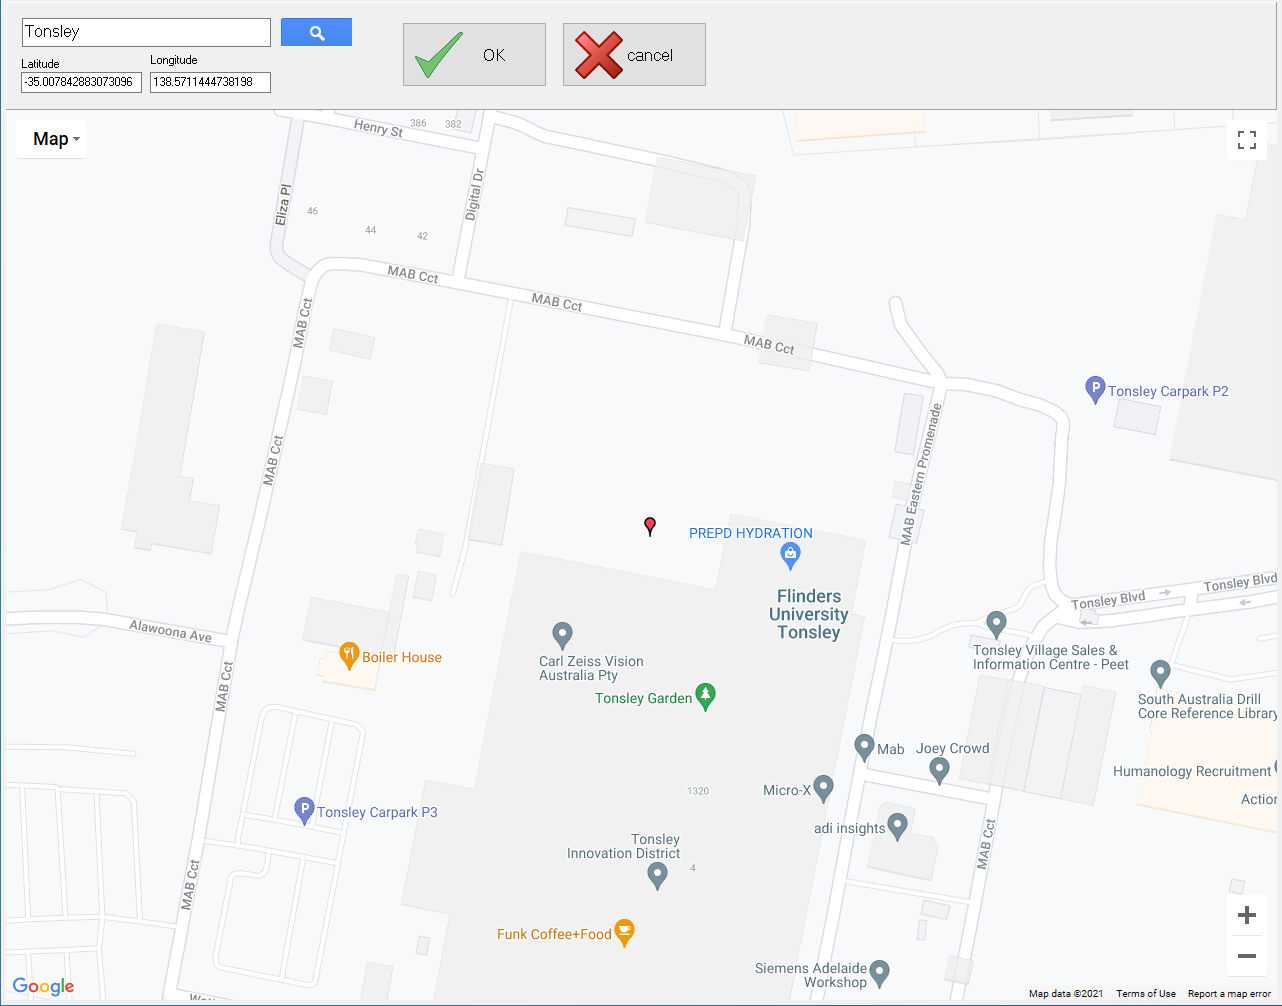
\includegraphics[width=12cm,keepaspectratio]{Figures/static coordinates setup.png}
        \caption{Using google maps within SatGen3 to choose a static coordinate to be used as desired spoof location}
    \label{fig:StaticCoordinate}
    \end{centering}
\end{figure}

\begin{figure}[ht]
    \begin{centering}
        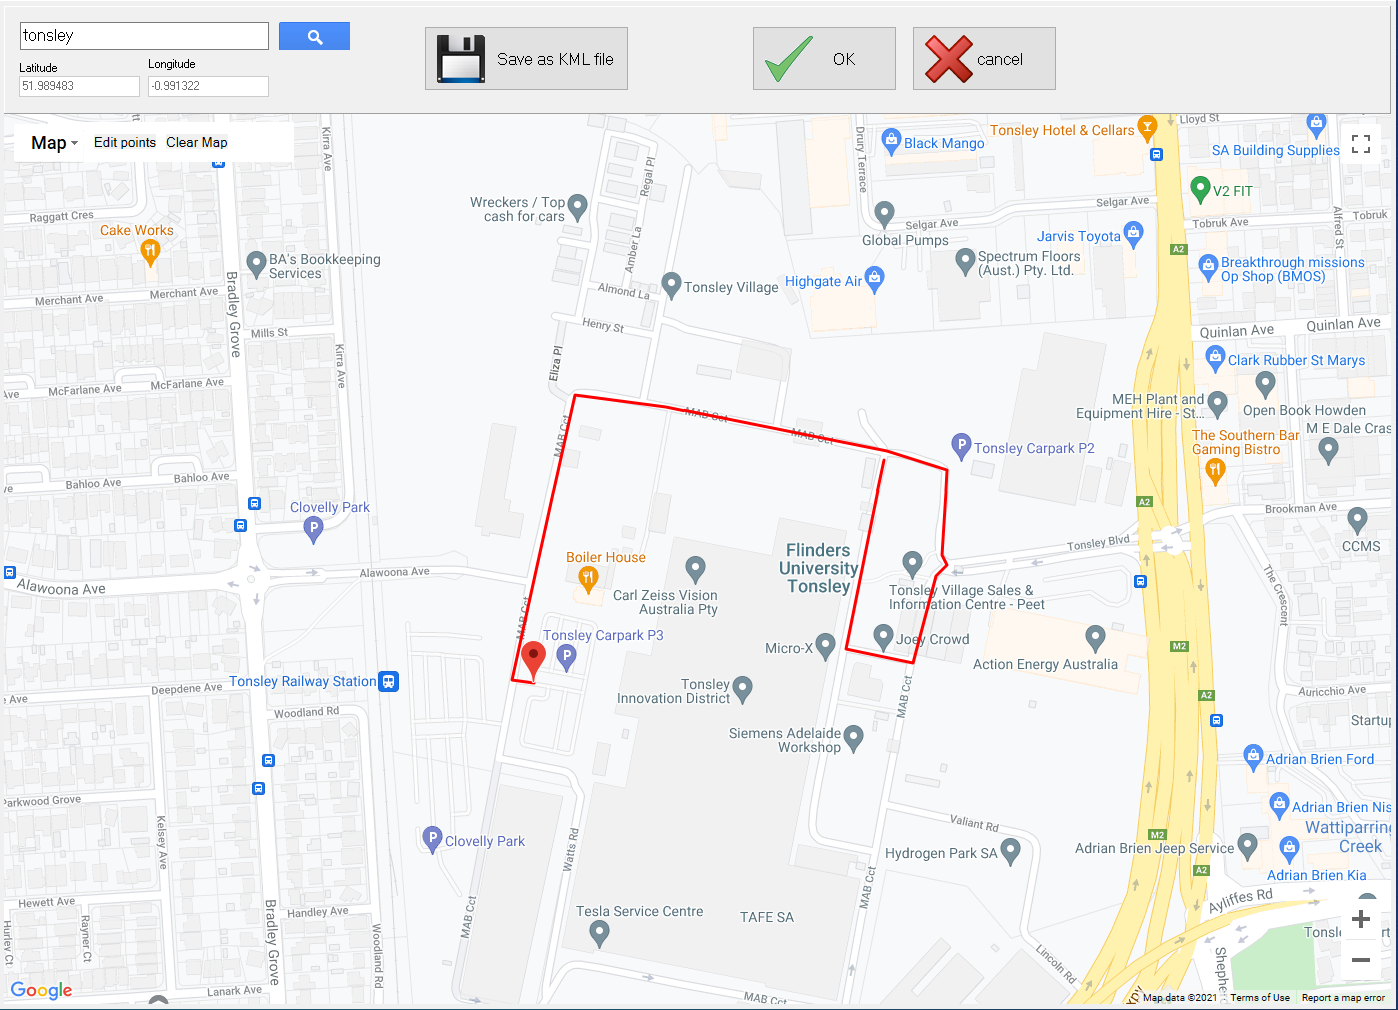
\includegraphics[width=12cm,keepaspectratio]{Figures/dynamic coordinates setup.png}
        \caption{Using google maps within SatGen3 to choose a set of coordinates to be used as desired spoof path for a dynamic spoof attack}
    \label{fig:DynamicCoordinate}
    \end{centering}
\end{figure}

\subsection{Generate NMEA File} \label{subsec:NMEAFile}
The coordinate and NMEA file creation step is essentially the same step within the SatGen3 software package. Once the coordinate or path was chosen, it was a matter of
choosing to save the output as a text file. An example of this is shown in Figure \ref{fig:StaticCoordinateNMEA}. In order to keep track of the source NMEA files and the
results files the following naming scheme was employed:

\begin{verbatim}
    YY_MM_DD_<static/dynamic>_LOCATION.nmea
    YY_MM_DD_<static/dynamic>_LOCATION.bin
    YY_MM_DD_<static/dynamic>_LOCATION.txt
\end{verbatim}

Where .nmea file was the source file, the .bin file was the signal binary file and the .txt file was the log file produced from the GPS receiver.

When generating a dynamic file there is an option to set the amount of "stationary" time. This will put a buffer of unmoving coordinates for a set amount of time. This
was used to allow the spoofing victim time to lock onto the spoofed signal before the simulated movement began.

To generate the binary bit stream for use with an SDR RF front end a GGA NMEA data stream was created using the SatGen3 software package. This NMEA stream was used to make
the binary file using the GPS-SDR-sim command line interface program. SatGen3 replaces the need for capturing the raw GNSS signals or GGA sentence stream thus increasing
the flexibility of scenarios that can be tested. Although there is no guarantee that the simulated stream of information is going to be correct. Thus a capture replay
attack should still be considered as more reliable.

\begin{figure}[!ht]
    \begin{centering}
        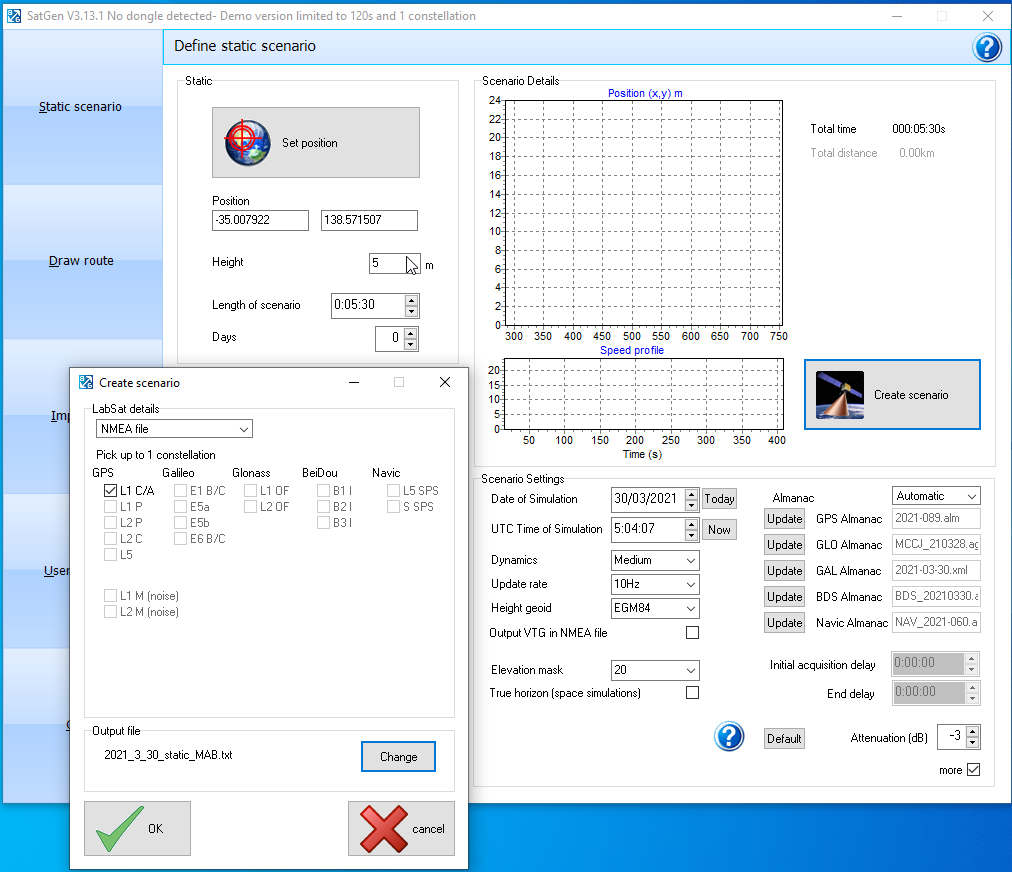
\includegraphics[width=12cm,keepaspectratio]{Figures/2021_03_30_static_MAB_setup.png}
        \caption{Using static coordinate to generate NMEA file}
    \label{fig:StaticCoordinateNMEA}
    \end{centering}
\end{figure}

\subsection{Download Ephemeris}
From the NASA website, hourly versions of the GPS constellation ephemeris, in the form of a RINEX file, are available. These are compiled into a daily file. These daily
files are available all the way from 1992. An account is required to access these files, but there are sample programs provided for retrieving
the files programatically using different methods. A script was generated that was able to get the latest version from the website using Python. The full version of this
script is shown in Appendix \ref{sec:EphemerisCode}. There were initially some
issues with getting the script to connect to the remote server to gain access to the files. It was found that there was a bug on Linux with a certain version of openssl.
A newer version was manually installed and this solved the issue.

The downloaded file was a compressed version of the text file, and thus it was required to be uncompressed using the tar program.

\subsection{Compile Signal Binary File}
GPS-SDR-sim compiles the signals into a 16bit data format where the first 8bits represents the in-phase data and the next 8 bits represents the Quadrature data information.
The minimum requirements to compile a binary file using GPS-SDR-SIM was a source coordinate in either ECEF or latitude/longitude format and the ephemeris for the desired date and time that the spoofer
will transmit. This did not need to match the date and time that the signal was being transmitted on. If the attack was to be a dynamic spoofing attack then it was
required that there be a "user motion file" or GGA sentence stream. This stream was required to be 10Hz. It was decided that even for static scenarios a GGA stream would
be used. This simplified the workflow overall. Using this method meant that the program was able to calculate the duration of the transmission itself. The output was
altered in order to conform with the naming convention stated in Section \ref{subsec:NMEAFile}. The sampling rate was also modified to be 2.5Msps instead of the default
2.6Msps.
When compiling some of the dynamic spoofing scenarios the maximum size was reached. This is a limit that is hardcoded when the GPS-SDR-sim program is compiled on the host
machine. Therefore, the program was cleanly recompiled in with the command to increase the maximum size of output file.

Using this information, the place, time and ephemeris the program is able to calculate which of the satellites will be in view and what their expected pseudoranges would
be. This is shown in Figure \ref{fig:sdrsimexample}.
The signal modulation is applied within the compilation of the file, simplifying the process of transmitting the file. 

\begin{figure}[!ht]
    \begin{centering}
        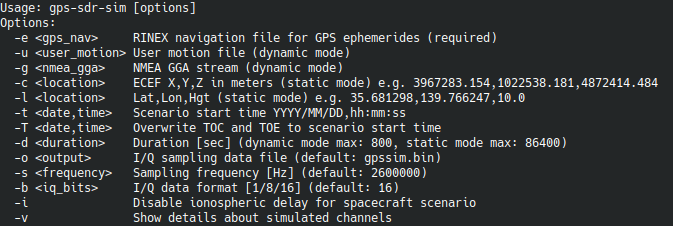
\includegraphics[width=14cm,keepaspectratio]{Figures/gps-sdr-sim options.png}
        \caption{Options available for compiling spoofed GPS signal using the GPS-SDR-SIM program}
    \label{fig:sdrsimoptions}
    \end{centering}
\end{figure}

\begin{figure}[!ht]
    \begin{centering}
        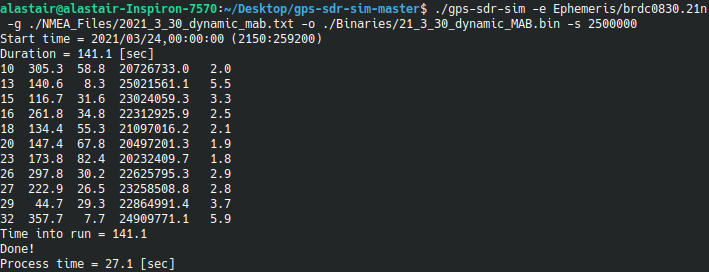
\includegraphics[width=14cm,keepaspectratio]{Figures/gps-sdr-sim running.png}
        \caption{Example of running GPS-SDR-sim with required arguments to generate dynamic spoof around the Tonsley MAB}
    \label{fig:sdrsimexample}
    \end{centering}
\end{figure}

\subsection{Transmit Signal}
Once the signal has been compiled into a binary file it is sent to the USRP SDR via GNURadio. GNURadio has an SDK that allows for text based programming. A script that was
capable of connecting to USRP devices automatically through the UHD daemon was distributed with the GPS-SDR-sim program. This was used to simplify the development
process. 

This was a simple program that connected the source file to the SDR via some simple blocks as shown in Figure \ref{fig:GNURadioSpoof}. The file is read 16bits at a time
into the "IShort to Complex" block. This converts the interleaved I/Q data into a complex file type which is then passed to the SDR via an amplifier block.

\begin{figure}[!ht]
    \begin{centering}
        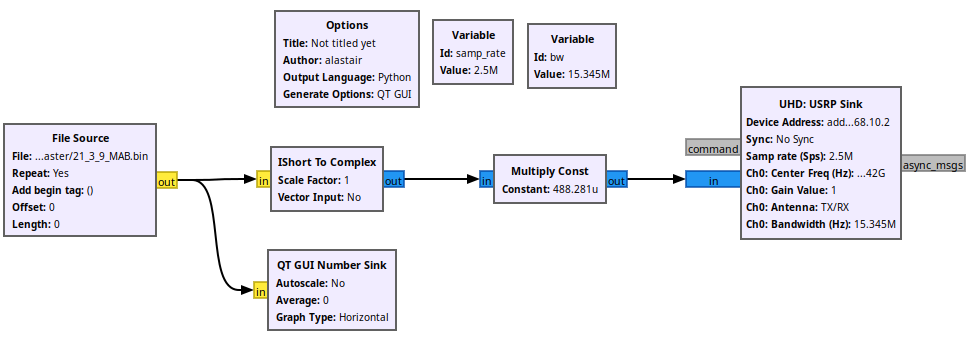
\includegraphics[width=14cm,keepaspectratio]{Figures/GNURadio_Spoofer.png}
        \caption{GNURadio flowchart for transmitting binary files with USRP}
    \label{fig:GNURadioSpoof}
    \end{centering}
\end{figure}

An important part of the transmission was that it needed to be performed within a Faraday cage for legal purposes. This was discussed in section \ref{sec:FaraCage}.

\subsection{Log GPS Data}
To log the transmitted GPS signals from the SDR a COTS receiver and a smartphone were set up. The COTS receiver has a USB interface that outputs a stream of NMEA
sentences at a 1Hz frequency. This can be modified to 5Hz, but this was not required for these experiments. Using a script the USB port was opened and logged to a text
file, see Appendix \ref{sec:GPSConnect}. The log file was passed as an argument and could be stored wherever it was needed. Each time a spoof attempt was made, the GPS
receiver was powered off to ensure there was not lock when starting the experiment. This ensured results were as consistent as possible.

When using a smartphone Android was required for logging since the OS allows access to the raw properties of the received signal. There is also an intuitive application
"GNSS Logger" that allows for comprehensive visualisation of current GNSS tracking as well as the ability to log data. This data was logged to a text file using a non
standard layout, but there was an option to log the NMEA sentences as well.  

\subsection{Generate Graphs}
Once there was a log file, graphs were generated to visualise the various parameters of the location resolution as interpreted by the receiver. 
The generation of the graphs that make up the results section was done in python and was based upon the NMEA sentences logged from the receivers. GPS receivers have the
ability to check the validity of signals they receive. When they are able to resolve a location the value of one of the fields within the RMC sentence is changed to
reflect this. The number of sentences before initial lock were counted. This was
used to determine the time to first fix of each test since it was known that the GPS receiver would output at 1Hz. Alterations would need to be made if the receiver was
outputting at a higher frequency. As such this should not be considered accurate and viewed as an estimate only.

The carrier to noise ratio graphs were generated directly from the output of the GSV sentences. The SVID and associated $\frac{C}{N_0}$ ratios were stored as the value in
a key value pair. The key was a timestamp used to ensure each sentence was represented.\\
The latitude and longitude were retrieved from the GGA sentences.

Using the NMEA stream created in section \ref{subsec:NMEAFile} a desired plot was put on both the static and dynamic graphs. For the static graphs this reference was also
used as the origin when calculating the error of the calculated location.

The error was calculated by finding the difference in latitude and longitude from the desired origin point and converting the $\Delta Lat$ and $\Delta Long$ into meters.
This assumes that the distances being dealt with are so small that they are essentially flat. Thus the equations can be simplified to remove any angles.

The earth is not perfectly spherical therefore when converting latitude and longitude into x and y coordinates in meters the average of the polar plane and equatorial
planes were taken, as shown in equation \ref{eq:EarthCircumference}. The $\Delta x$ and $\Delta y$ values from Equation \ref{eq:deltaX} and \ref{eq:deltaY} represent
the error of the coordinate in the $x$ and $y$ direction respectively. \\
When finding the total error value the law of Haversines was used. 

\begin{equation} 
    \begin{split} \label{eq:EarthCircumference}
        C_{Polar} = 40007.863 km \\ 
        C_{Equatorial} = 40075.017 km
    \end{split}
\end{equation}

\begin{equation} \label{eq:deltaX}
    \Delta x = \Delta Lat \times \frac{C_{Polar}}{\frac{2}{180}} \times 1000 m
\end{equation}

\begin{equation} \label{eq:deltaY}
    \Delta y = \Delta Long \times \frac{C_{Equatorial}}{\frac{4}{90}} \times 1000 m
\end{equation}

\begin{equation} \label{eq:Haversine}
    d = 2r \arcsin\left(\sqrt{\sin^2\left(\frac{\phi_2 - \phi_1}{2}\right) + \cos\left(\phi_1\right)\cos\left(\phi_2\right)\sin^2\left(\frac{\lambda_2 - \lambda_1}{2}\right)}\right)
\end{equation}
 
Below (Listing \ref{list:pythonHaversines}) is the implementation of the law of Haversines in python used for the calculation of distance between two latitude and longitude points. The output of the function was stored
into an array and used to graph the total error over time.

% \begin{verbatim}
%     def latlon2m(lat1, long1, lat2, long2):
%         r = 6371000  
%         dLat = radians(lat2) - radians(lat1)
%         dLong = radians(long2) - radians(long1)
%         a = math.sin(dLat/2) * math.sin(dLat/2) + 
%             math.cos(radians(lat1)) * math.cos(radians(lat2)) *
%             math.sin(dLong/2) * math.sin(dLong/2)
%         d = 2*r*math.asin(math.sqrt(a))
%         return d
% \end{verbatim}

\begin{lstinputlisting}[language=Python, label=list:pythonHaversines, caption=Python implementation of the law of Haversines used to calculate the distance between two points on a sphere, firstline=23, lastline=29]{NMEAParse.py}
\end{lstinputlisting}

There is a PC companion application for the GNSS Logger app that allows for comprehensive
graphing and reports to be generated for a particular log file.


\section{Experiments}
\subsection{Static Spoofing}
Within this thesis static spoofing is defined as producing a signal that produces a calculated location that does not change over time. While in practise there was some
minor movement caused by the uncertainty in trilateration, this change in position is minor and within the range of error of GPS positioning.
Using the SatGen3 software a location was chosen as the spoof location. After setting the desired time and date of spoofing the scenario was created. This 

\subsection{Dynamic Spoofing}
Dynamic spoofing refers to the production of a signal that when used to calculate position, will be shown to change over time. The path traced by the receiver will be
set at the time of production of the binary file, but there will be perceived motion.

\subsection{Real-Time Spoofing}
Due to time constraints a real-time algorithm was not produced as part of this project. However, utilising the open source projects that have been used to complete this
thesis it would be probable to be able to create a real time spoofing device that would be able to react to the positional changes of the receiver instead of following a
pre-determined path when generating the binary file. The signals generation algorithm could be ported to a GNURadio block in C++ to allow for easy access to real-time GPS
signal spoofing. If an SDR is a full duplex radio, such is the case for the USRP N210, then one port can be receiving the real GNSS signal and the other can be
transmitting the spoofed signal. Care would need to be taken in the set up of this arrangement since any transmitted signal would also be picked up by the receiving
antenna. Therefore a directional transmitting antenna and physical distance should be employed to allow for legitimate GNSS signals to reach the receiver port. 